% Created 2017-04-11 Tue 08:53
\documentclass[17pt,aspectratio=169]{beamer}
\usepackage[utf8]{inputenc}
\usepackage[T1]{fontenc}
\usepackage{fixltx2e}
\usepackage{graphicx}
\usepackage{longtable}
\usepackage{float}
\usepackage{wrapfig}
\usepackage{rotating}
\usepackage[normalem]{ulem}
\usepackage{amsmath}
\usepackage{textcomp}
\usepackage{marvosym}
\usepackage{wasysym}
\usepackage{amssymb}
\usepackage{hyperref}
\tolerance=1000
\usepackage{minted}
\institute{Department of Microbiology\\ School of Natural Sciences\\ National University of Ireland, Galway}
\fontfamily{pag}
\usepackage{libertine}
\renewcommand*\familydefault{\sfdefault}
\newcommand{\bt}{\textasciigrave}
\usepackage{xcolor}
\def \ttilde {\raisebox{-.6ex}\textasciitilde~}
\setlength\parindent{0pt} %set indent to zero
\setlength{\parskip}{1em}
\definecolor{bg}{HTML}{B1F4A0}
\usepackage{tcolorbox}
\usepackage{etoolbox}
\BeforeBeginEnvironment{minted}{\begin{tcolorbox}\scriptsize}%
\AfterEndEnvironment{minted}{\normalsize\end{tcolorbox}}%
\usepackage{geometry}
\usepackage[colorlinks = true, linkcolor = blue, urlcolor  = blue, citecolor = blue, anchorcolor = blue]{hyperref}
\let\oldv\verbatim
\let\oldendv\endverbatim
\def\verbatim{\par\setbox0\vbox\bgroup\scriptsize\oldv}
\def\endverbatim{\oldendv\egroup\fboxsep0pt \noindent\colorbox[gray]{0.8}{\usebox0}\par}
\usepackage{array, booktabs, xcolor, tikz}
\makeatletter
\renewcommand{\itemize}[1][]{%
\beamer@ifempty{#1}{}{\def\beamer@defaultospec{#1}}%
\ifnum \@itemdepth >2\relax\@toodeep\else
\advance\@itemdepth\@ne
\beamer@computepref\@itemdepth% sets \beameritemnestingprefix
\usebeamerfont{itemize/enumerate \beameritemnestingprefix body}%
\usebeamercolor[fg]{itemize/enumerate \beameritemnestingprefix body}%
\usebeamertemplate{itemize/enumerate \beameritemnestingprefix body begin}%
\list
{\usebeamertemplate{itemize \beameritemnestingprefix item}}
{%
\setlength\topsep{-2pt}%NEW
\setlength\partopsep{-2pt}%NEW
\setlength\itemsep{0pt}%NEW
\def\makelabel##1{%
{%
\hss\llap{{%
\usebeamerfont*{itemize \beameritemnestingprefix item}%
\usebeamercolor[fg]{itemize \beameritemnestingprefix item}##1}}%
}%
}%
}
\fi%
\beamer@cramped%
\raggedright%
\beamer@firstlineitemizeunskip%
}
\makeatother
\setbeamerfont{frametitle}{size=\normalsize}
\usepackage{graphicx}
\usetikzlibrary{arrows, calc, spy}
%%%%% %%%%% %%%%% %%% %%%%  for pretty headers with pictures
\addtobeamertemplate{frametitle}{}{%
\begin{tikzpicture}[remember picture,overlay]
\node[anchor=north east,yshift=2pt] at (current page.north east) {
\includegraphics[height=0.75cm]{../stock_logos/nuig_rounded.png}  \hspace*{.05cm} 
\includegraphics[height=.74cm, trim= 0cm 0.0cm 0.0cm 0cm]{../stock_logos/jhi_rounded.png}};
\end{tikzpicture} \vskip -1.1cm}
\addtobeamertemplate{footnote}{\tiny}{} %\vspace{2ex}}
\usetheme{default}
\author{Nicholas Waters \linebreak \\ \footnotesize  Ashleigh Holmes, Florence Abram,  Leighton Pritchard, and Fiona Brennan \vskip -1cm}
\date{\today}
\title{Comparative Genomics of Soil-persistant \emph{E. coli}}
\hypersetup{
  pdfkeywords={},
  pdfsubject={},
  pdfcreator={Emacs 24.4.4 (Org mode 8.2.10)}}
\begin{document}

\maketitle
\begin{frame}[label=sec-1]{Introduction}
\begin{itemize}
\item Overview of soil-persistent \emph{E. coli}
\item Research questions
\item Experimental design
\item Results
\item Next Steps
\end{itemize}
\end{frame}

\begin{frame}[label=sec-2]{\emph{E. coli}: commensal or pathogen?}
\begin{itemize}
\item Gram negative
\item Beneficially occurs in the gut
\item Can infect gi and urinary tracts
\item Health burden: \textasciitilde{}5 million DALY         \footnote{Image source: NDSU}
\item Used as contaminaiton indicator
\end{itemize}

\begin{tikzpicture}[remember picture,overlay]
    \node[xshift=-5.35em,yshift=-4cm] at (current page.north east) {
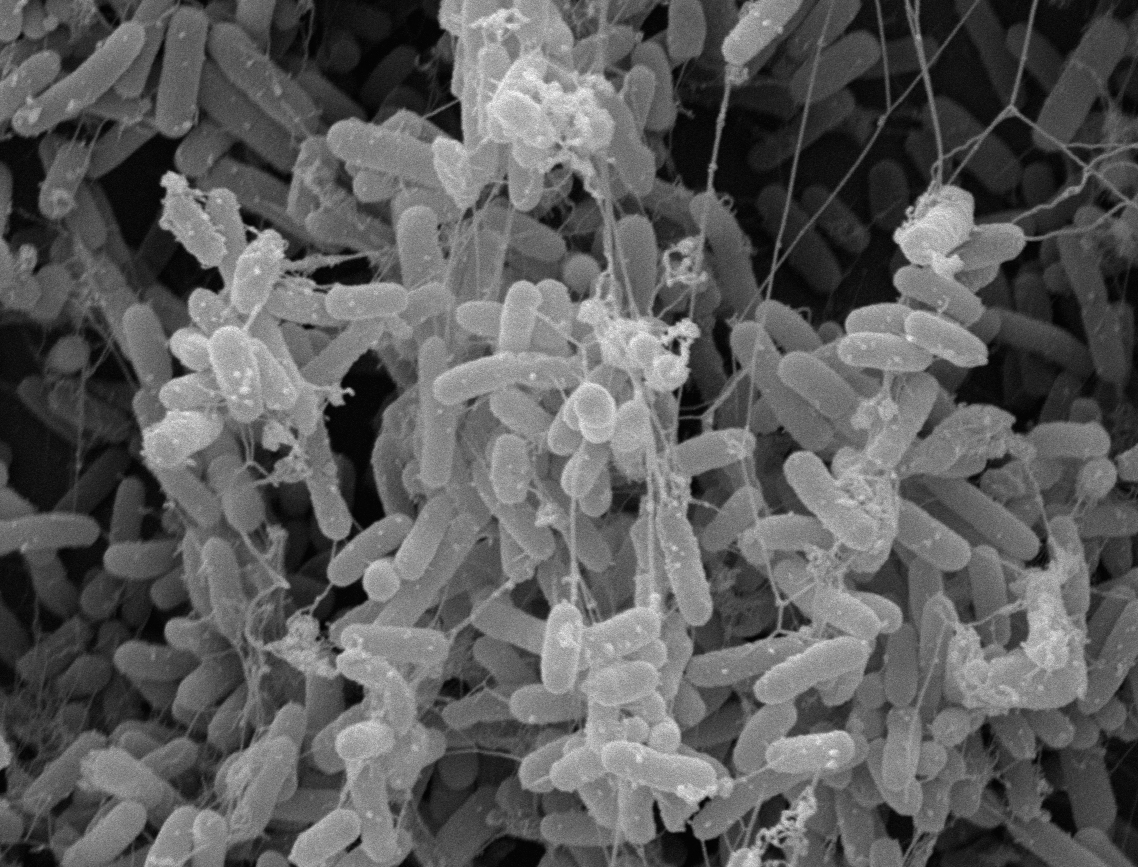
\includegraphics[width=.35\textwidth]{./20170411_environ_figs/biofilm.jpeg}
};
\end{tikzpicture}
\end{frame}


\begin{frame}[label=sec-3]{A Brief History of Soil-persistent E. coli}
\newcommand\ytl[2]{
\parbox[b]{4em}{\hfill{\color{cyan}\bfseries\sffamily #1}~$\cdots\cdots$~}\makebox[0pt][c]{$\bullet$}\vrule\quad \parbox[c]{24em}{\vspace{7pt}\color{red!40!black!80}\raggedright\sffamily #2\\[7pt]}\\[-3pt]}
\begin{table}{\small
% \caption{A Brief Literature Review}
 \vskip -5mm
\centering
\begin{minipage}[t]{\linewidth}
\color{gray}
\rule{\linewidth}{1pt}
\ytl{1886}{Escherich: Discovery of \textit{E. coli}}
\ytl{1948}{Bardsley: Soil may act as reservoir for \textit{E. coli}}
\ytl{1963}{W. and J. Boyd: Cold persistence observed }
%\ytl{1967}{Klein, et al: Die-off related to metabolism rates}
\ytl{1972}{Evans, et al: Drainage related to coliform counts} % and slurry spreading
\ytl{1988}{Fujioka and Shizumura: Alternative indicators suggested }
%\ytl{1992}{Tsai, et al: PCR detection of from soil}
\ytl{1997}{Texier, et al: Stable populations exist in alpine grasslands}
%\ytl{1998}{Byappanahalli and Fujioka: Soil extracts as growth media}
\ytl{2003}{Byappanahalli, et al: Soil persistence is widespread }
\ytl{2010}{Brennan, et al: Persistence in maritime temperate soils}
\bigskip
\rule{\linewidth}{1pt}%
\end{minipage}%
}
\end{table}
\end{frame}

\begin{frame}[label=sec-4]{Research Questions}
\begin{block}{Genomic Context}
\begin{itemize}
\item Are soil-persistent \emph{E. coli} related?
\item Do soil-persistent \emph{E. coli} possess certain traits?
\end{itemize}
\end{block}
\begin{block}{Virulence}
\begin{itemize}
\item Are soil-persistent strains pathogenic?
\end{itemize}
\end{block}
\end{frame}

\begin{frame}[label=sec-5]{Experimental Design: Background}
Ryan and Fanning: Effects of N and slurry on soils
\begin{itemize}
\item Isolate and protect grassland soil columns
\item Apply treatment, test leachate
\item Last application of slurry in 1998
\end{itemize}
Brennan, et al: Pathogen survival and transport in soils
\begin{itemize}
\item Two conditions: Cattle slurry and  control
\item Compare coliform counts in leachate
\end{itemize}
\end{frame}
\begin{frame}[label=sec-6]{Experimental Design: Current}
\begin{itemize}
\item Collect leachate from control lysimeters
\item Enrich for \emph{E. coli}
\item Purify, sequence genomes
\item Compare genomics of soil strains to wider \emph{E. coli} pangenome
\end{itemize}
\end{frame}

\begin{frame}[label=sec-7]{Soil Samples}
\begin{figure}[htb]
\centering
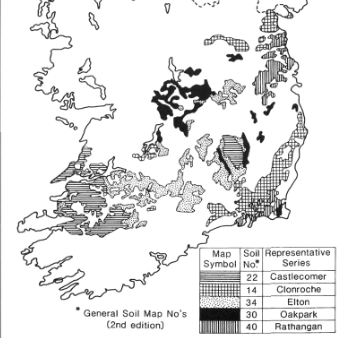
\includegraphics[width=.55\textwidth]{/home/nicholas/GitHub/FB/Ecoli_comparative_genomics/doc/presentations/MyNUIG(mnuigtheme)/lys_photos/RyanFanning1.png}
\caption{\label{fig:lys3}Lysimeter}
\end{figure}
\footnotemark[1]{}
\end{frame}

\begin{frame}[label=sec-8]{Lysimeters}
\begin{figure}[htb]
\centering
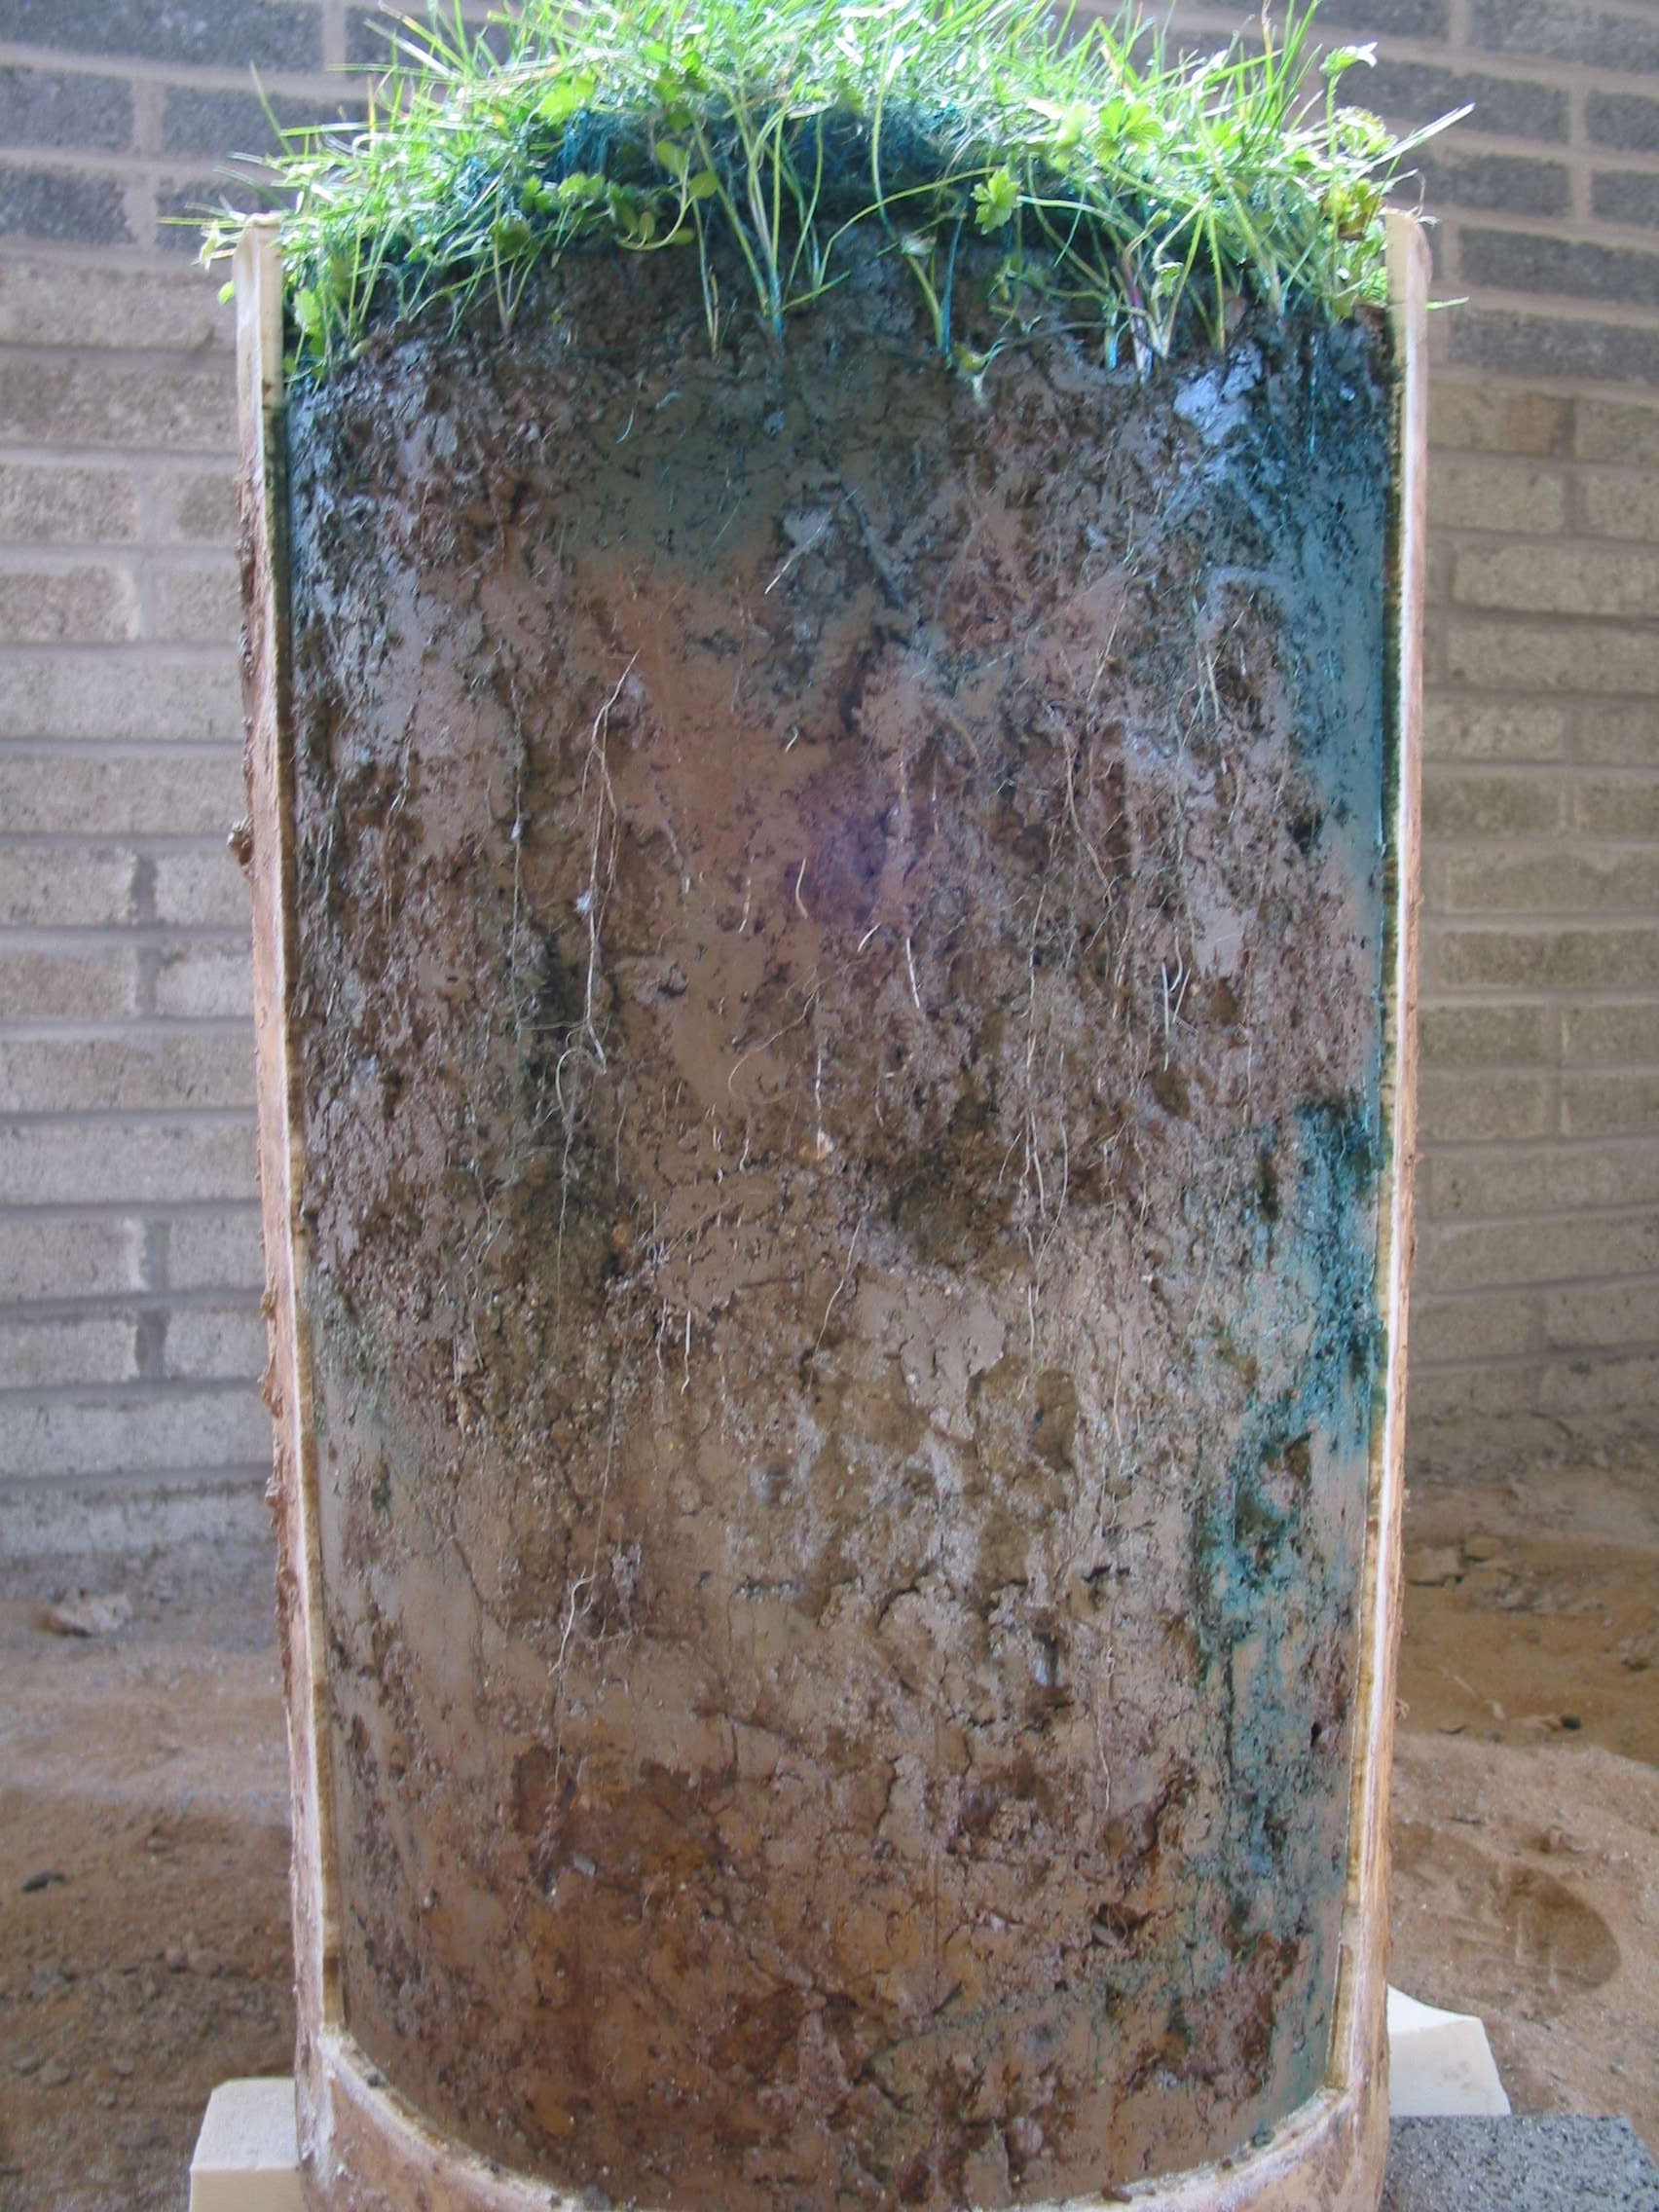
\includegraphics[width=6cm]{/home/nicholas/GitHub/FB/Ecoli_comparative_genomics/doc/presentations/MyNUIG(mnuigtheme)/lys_photos/rath2.jpg}
\caption{\label{fig:lys1}Lysimeter}
\end{figure}
\end{frame}

\begin{frame}[label=sec-9]{Lysimeters}
\begin{figure}[htb]
\centering
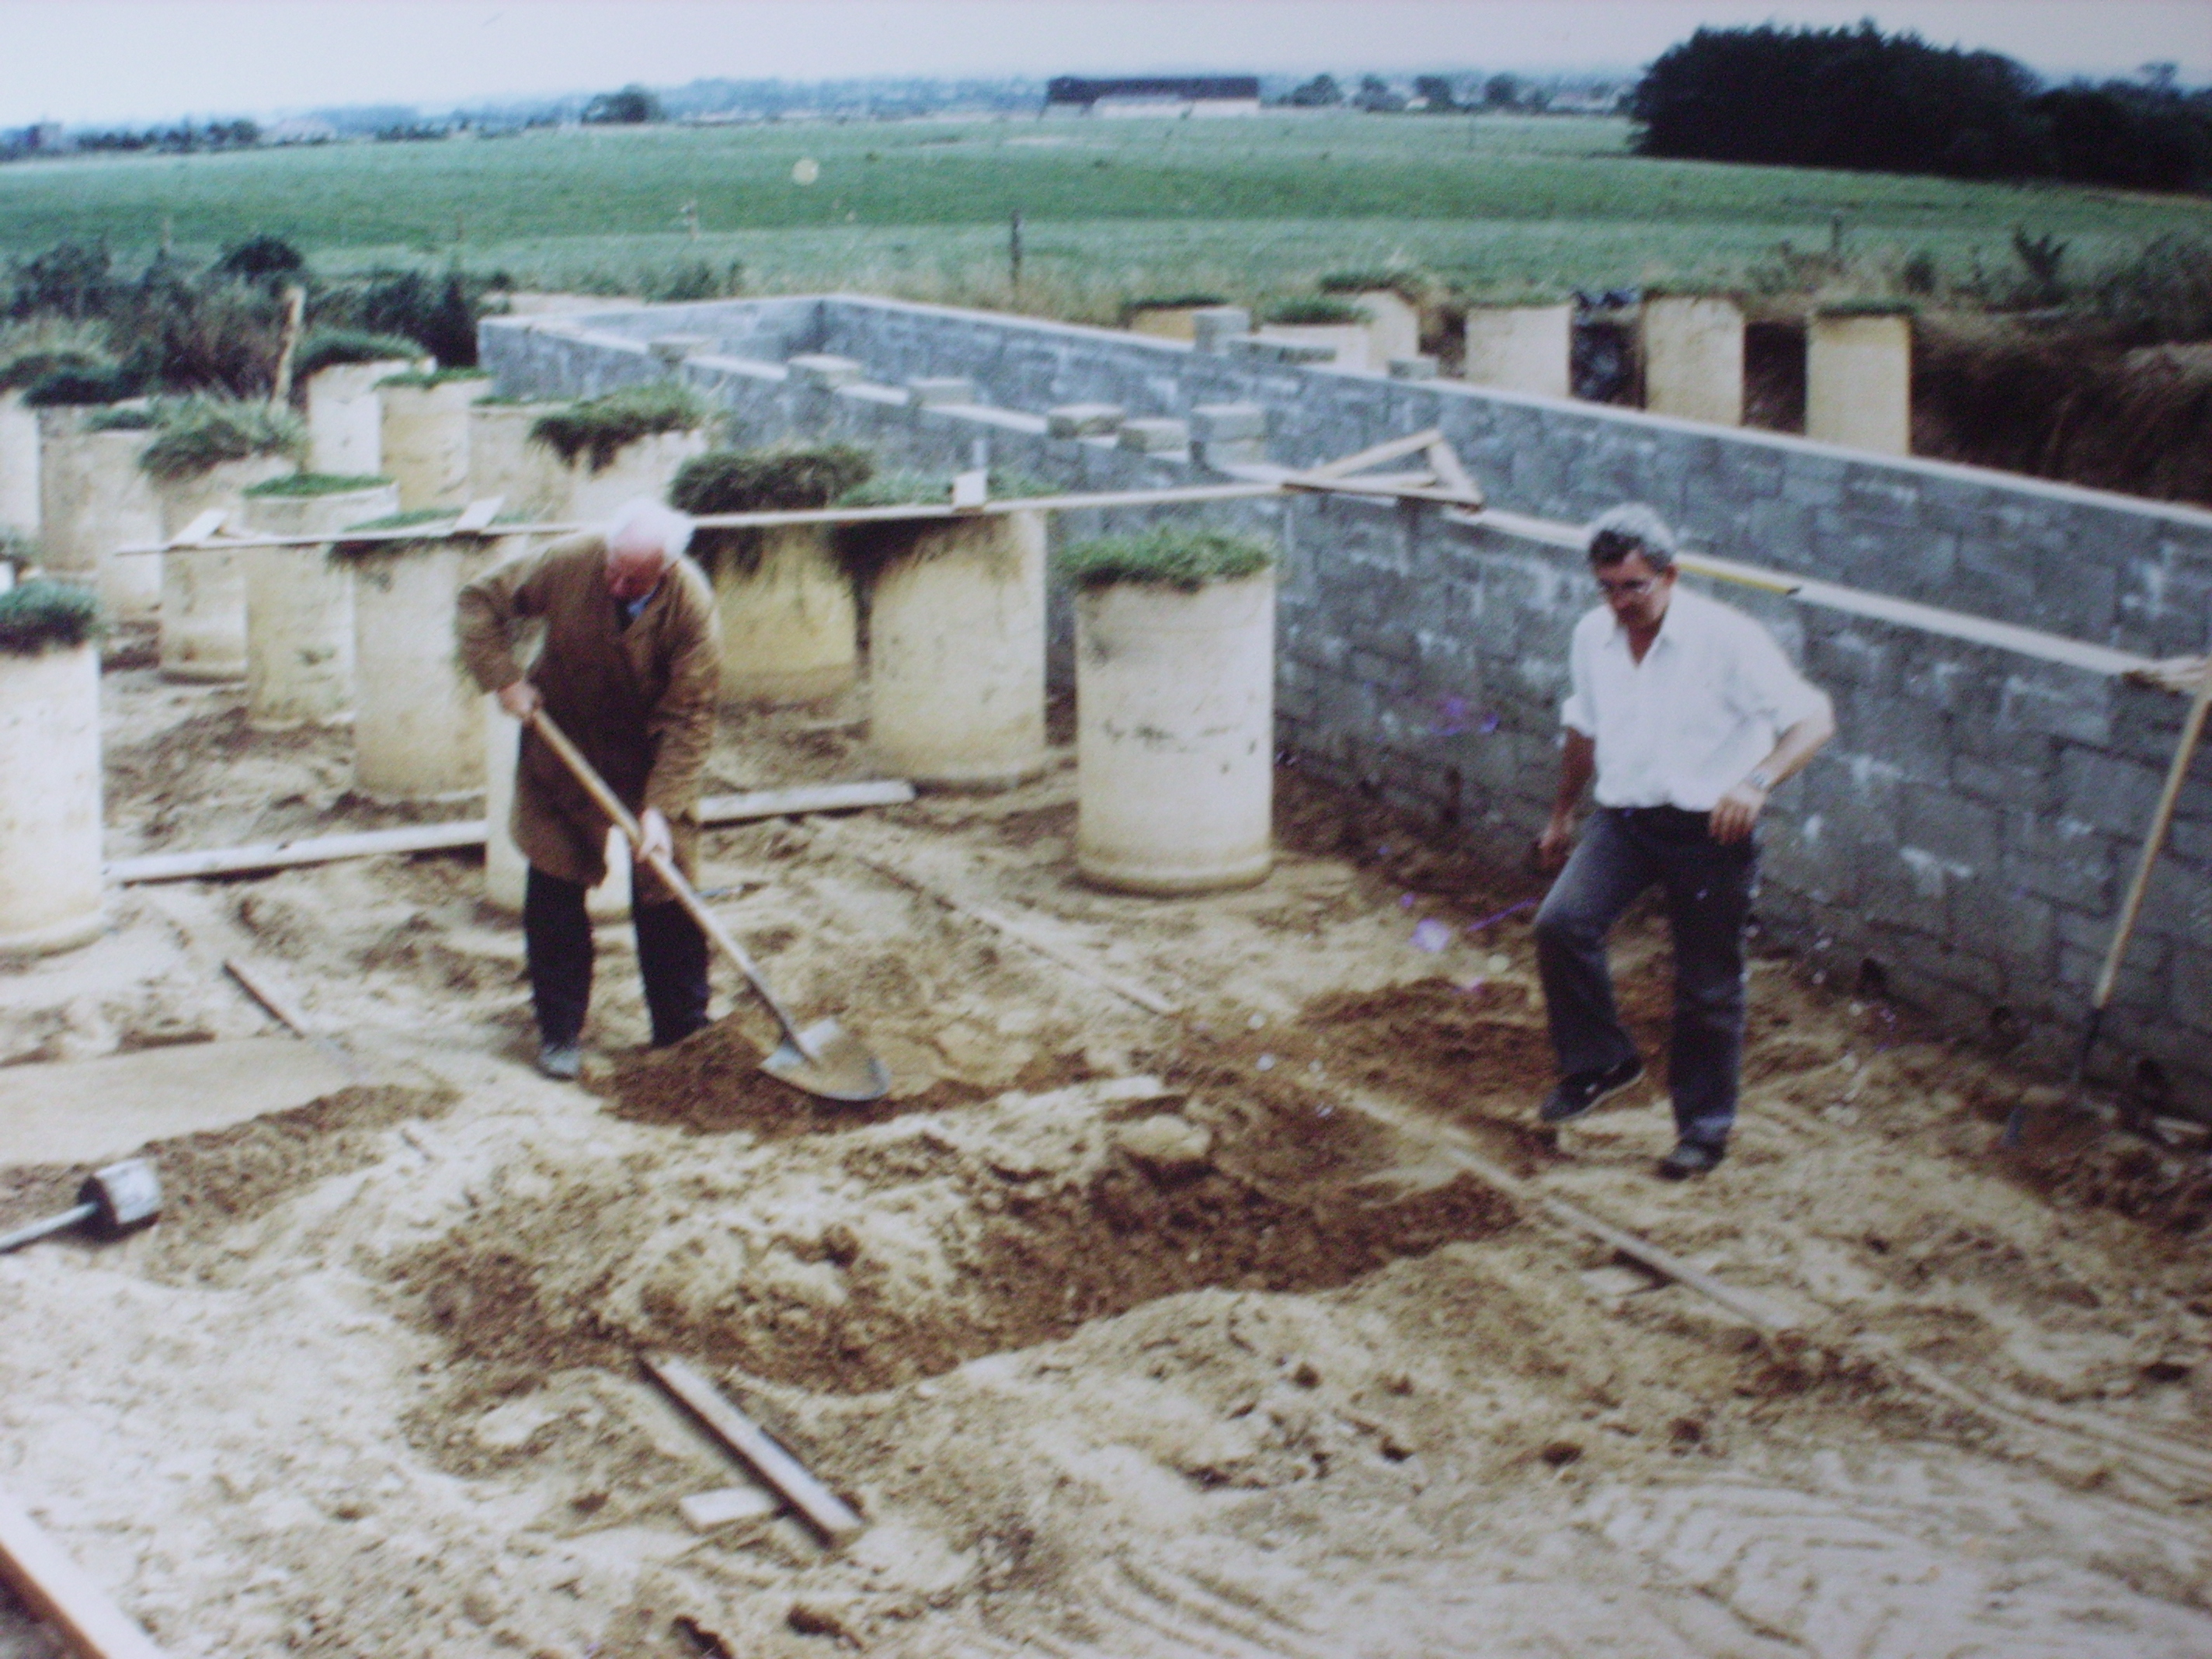
\includegraphics[width=10cm]{/home/nicholas/GitHub/FB/Ecoli_comparative_genomics/doc/presentations/MyNUIG(mnuigtheme)/lys_photos/IMGP0225.JPG}
\caption{\label{fig:lys2}Lysimeter}
\end{figure}
\end{frame}

\begin{frame}[label=sec-10]{Lysimeters}
\begin{figure}[htb]
\centering
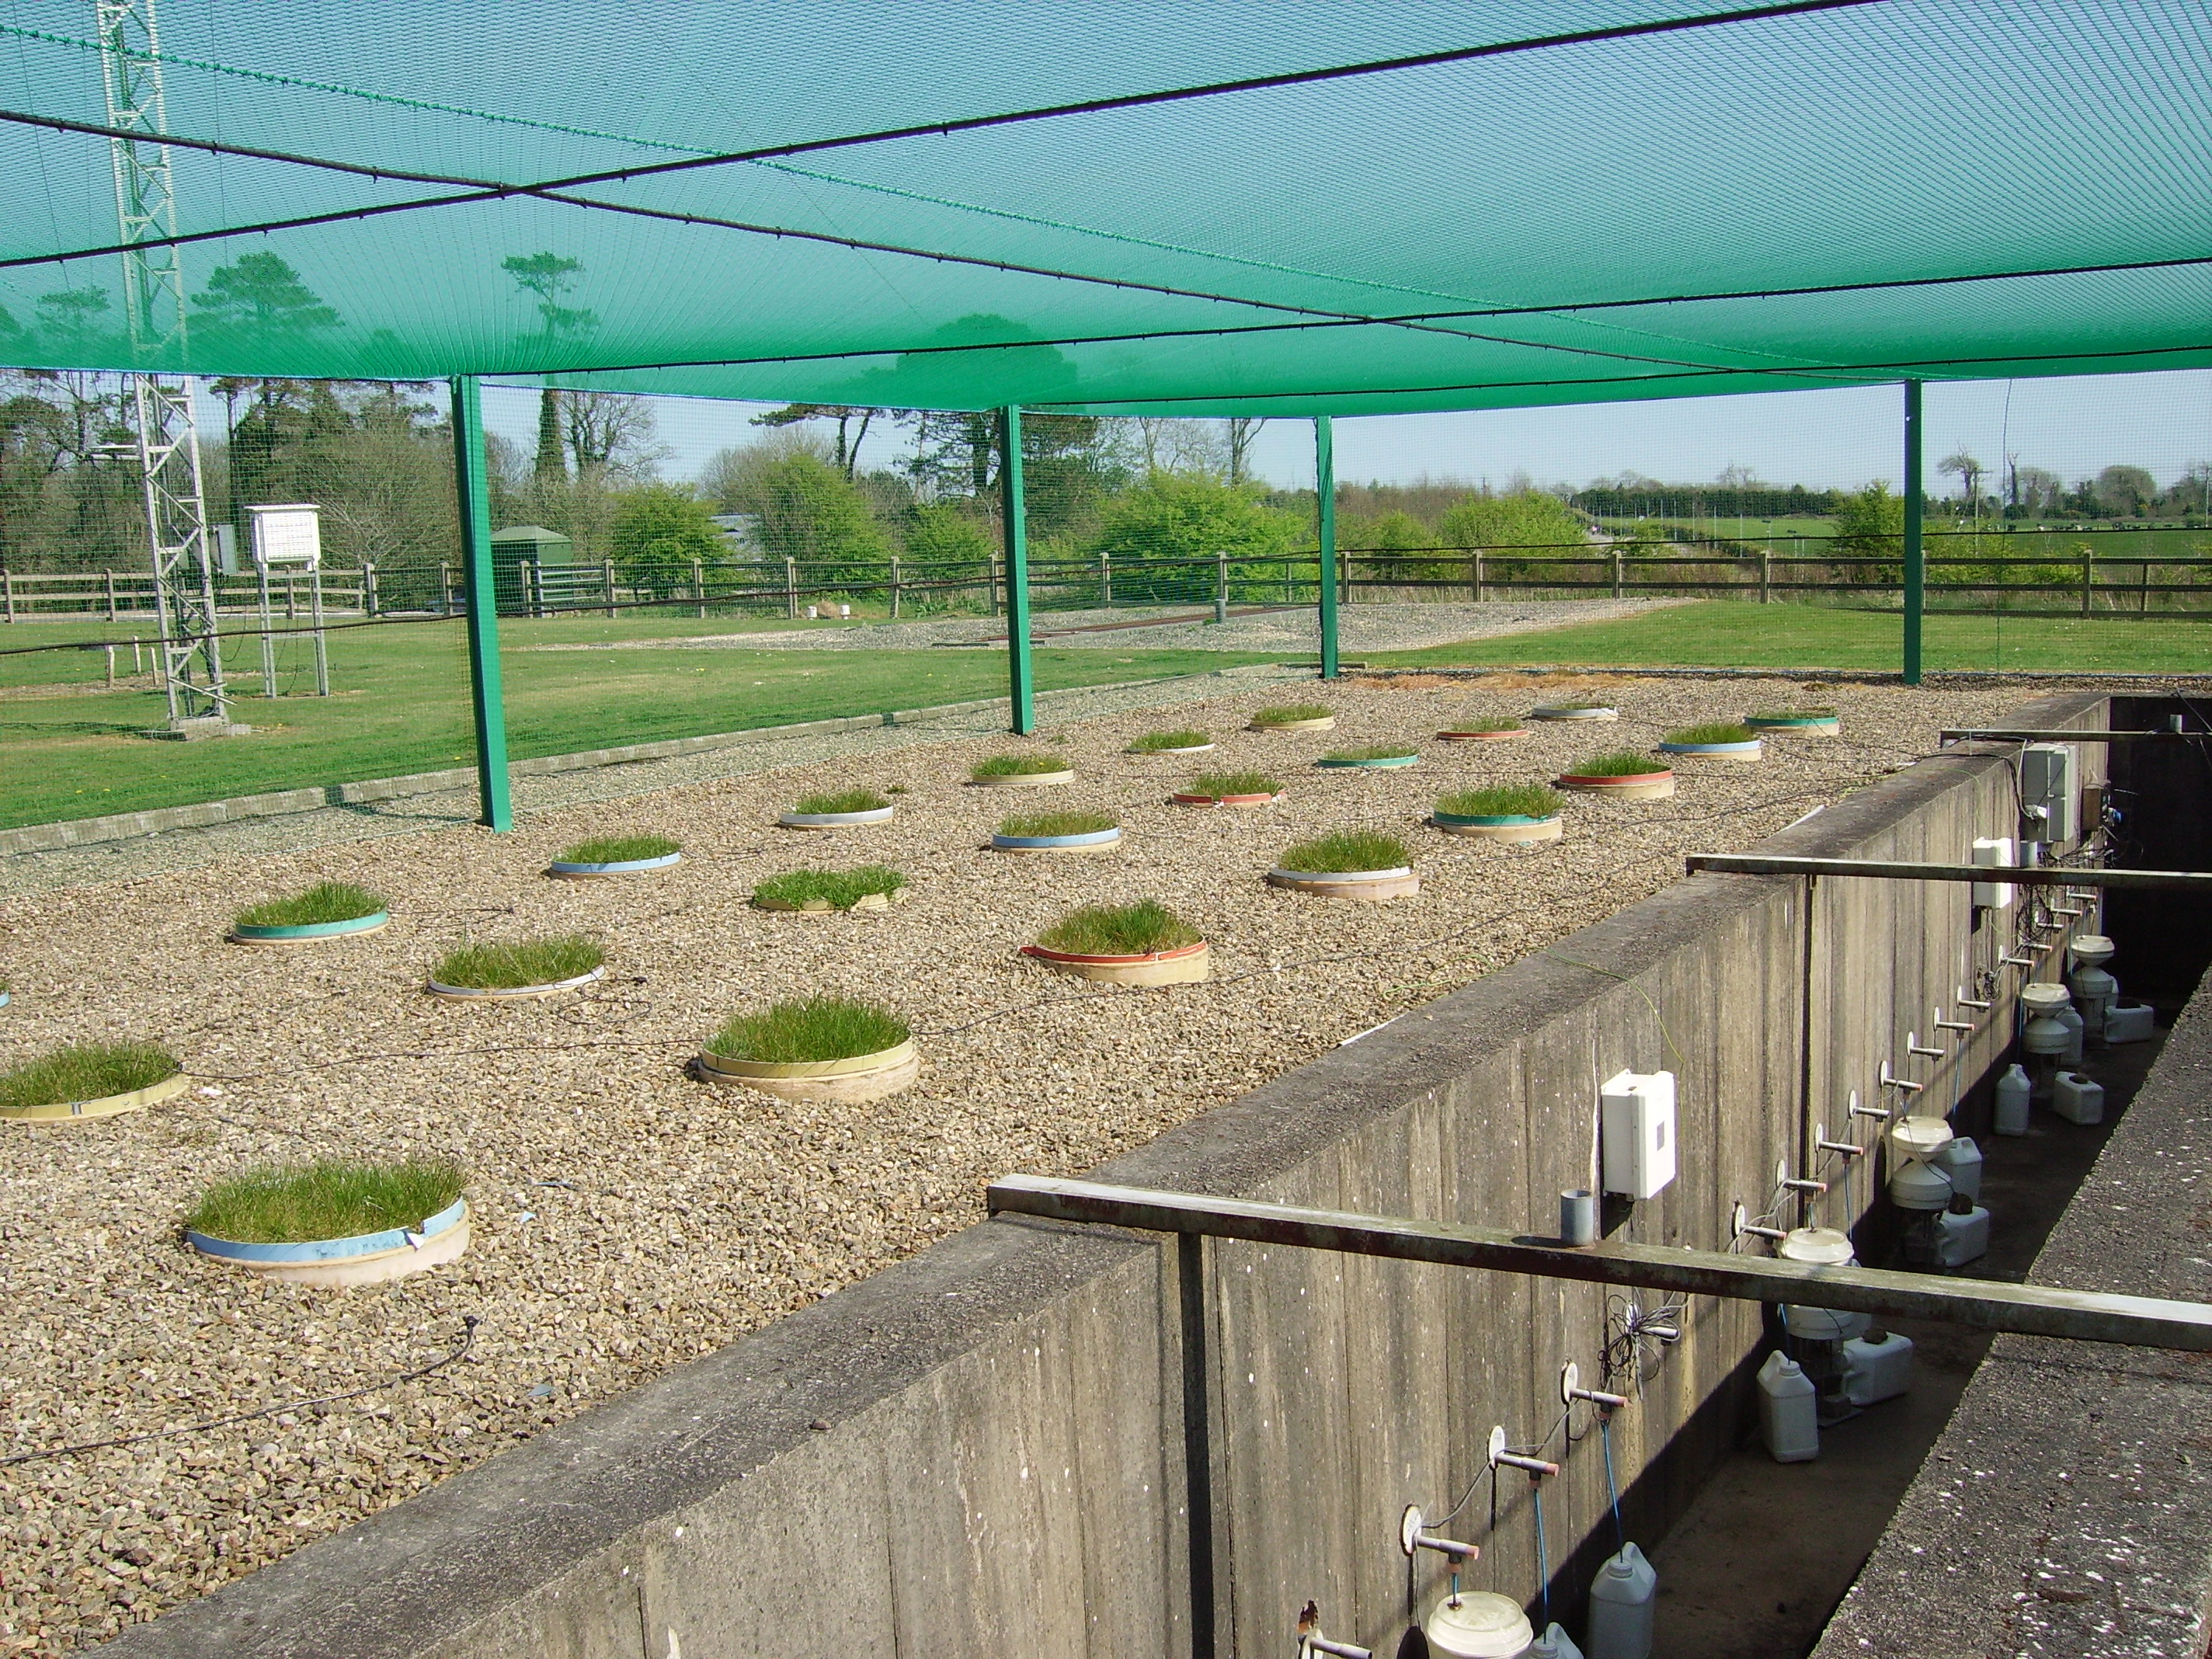
\includegraphics[width=10cm]{/home/nicholas/GitHub/FB/Ecoli_comparative_genomics/doc/presentations/MyNUIG(mnuigtheme)/lys_photos/IMGP0305.JPG}
\caption{\label{fig:lys3}Lysimeter}
\end{figure}
\end{frame}

\begin{frame}[label=sec-11]{Lysimeters}
\begin{figure}[htb]
\centering
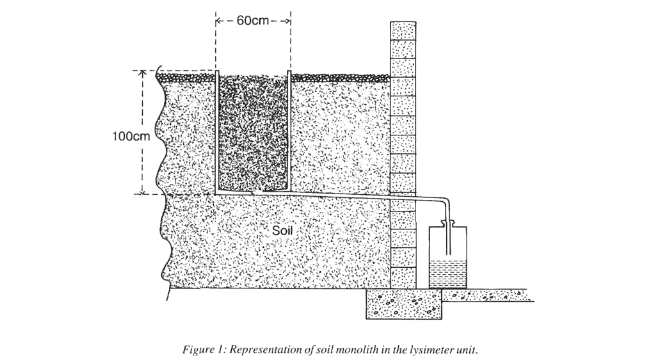
\includegraphics[width=\textwidth]{/home/nicholas/GitHub/FB/Ecoli_comparative_genomics/doc/presentations/MyNUIG(mnuigtheme)/lys_photos/RyanFanning2.png}
\caption{\label{fig:lys3}Lysimeter}
\end{figure}
\end{frame}



\begin{frame}[label=sec-12]{Workflow}
\begin{figure}[htb]
\centering
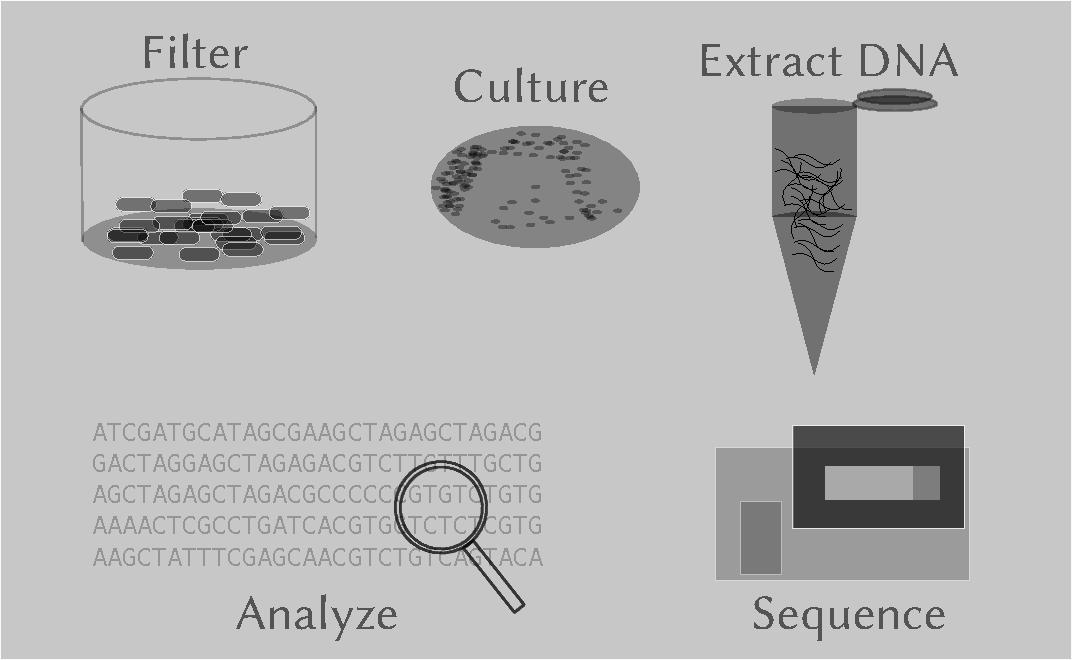
\includegraphics[width=.86\textwidth]{./frequentFigs/workflow_v1.pdf}
\caption{\label{fig:workflow}workflow}
\end{figure}
\end{frame}

\begin{frame}[label=sec-13]{Genomic Context}
\begin{itemize}
\item 202 isolates sequenced
\item 153 true \emph{E. coli} passed QC
\item All Clermont phylotypes represented
\end{itemize}
\vskip .5mm
\begin{itemize}
\item Diverse phenotypes
\begin{itemize}
\item curli
\item metabolism
\item biofilm
\end{itemize}
\end{itemize}

\begin{tikzpicture}[remember picture,overlay]
    \node[xshift=-3.5cm,yshift=-4.5cm] at (current page.north east) {
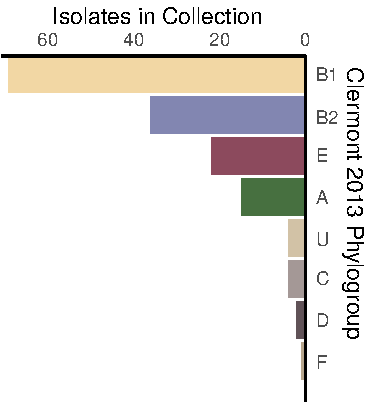
\includegraphics[width=.3\textwidth]{./20170411_environ_figs/Phylogroups.pdf}
};
\end{tikzpicture}
\end{frame}

\begin{frame}[label=sec-14]{Genomic Context}
\begin{tikzpicture}[remember picture,overlay]
    \node[xshift=-8cm,yshift=-4.8cm] at (current page.north east) {
\includegraphics[width=.55\textwidth]{../../posters/utrecht2016/figs/ANIm_percentage_identity_edited.pdf}
};
\end{tikzpicture}
\end{frame}


\begin{frame}[label=sec-15]{Virulence}
\begin{itemize}
\item Search literature for genes implicated in virulence
\item Select representative sequences for \textasciitilde{}50 virulence factors
\item Use reciprocal translated blast to find occurrences
\item Filter results, visualize
\end{itemize}
\end{frame}

\begin{frame}[label=sec-16]{Virulence Results}
%\begin{tikzpicture}[remember picture, overlay]
%    \node[xshift=-5cm,yshift=-4.8cm] (innerimage) at (current page.north east){
\hspace{1.5cm}\begin{tikzpicture}[spy using outlines={red,square,magnification=4, size=3.5cm,connect spies}]
    % Use Wikipedias image of the day
    \node[anchor=south west,inner sep=0] (image) at (0,0){
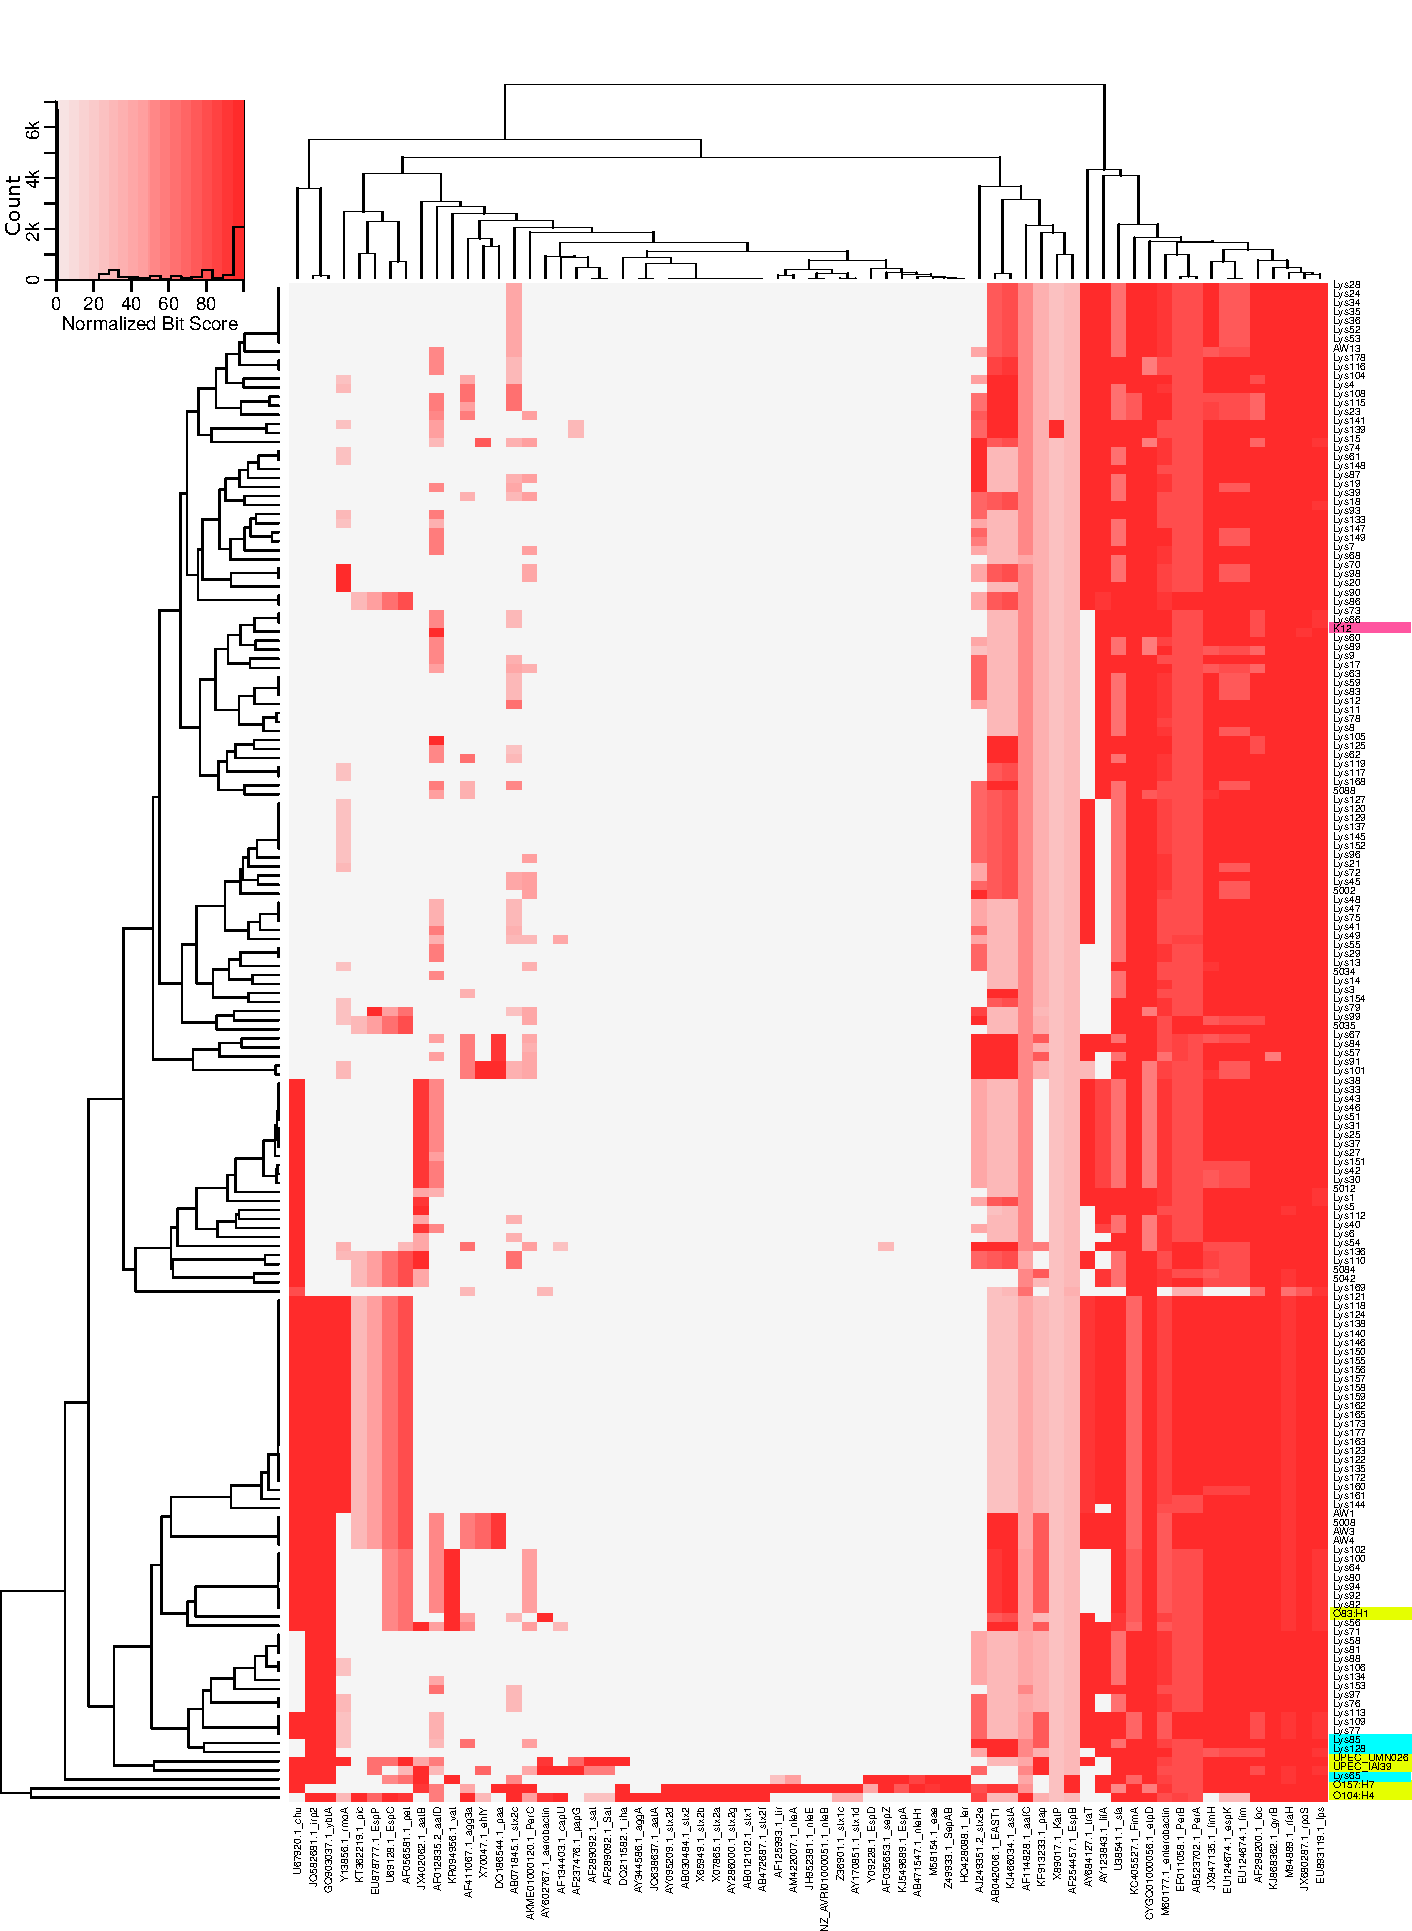
\includegraphics[width=5cm]{./frequentFigs/20161122170535_blast_virulence_parser_output_heatmap_edited3.pdf}};
%        \begin{scope}[x={(image.south east)},y={(image.north west)}]
%        \foreach \x in {0,1,...,9} { \node [anchor=north] at (\x/10,0) {0.\x}; }
%        \foreach \y in {0,1,...,9} { \node [anchor=east] at (0,\y/10) {0.\y}; }
%        \end{scope}
    \spy on ($0.9*(image.south east)+0.19*(image.west)$) in node at ([xshift=-2cm]image.west);
%%%%%%%    \spy on ($0.55*(image.south east)+0.95*(image.north west)$) in node at ([yshift=1cm]image.north);
%\end{tikzpicture}};
\end{tikzpicture}
\end{frame}

\begin{frame}[label=sec-17]{Conclusions about Soil-persistent \emph{E. coli}}
\begin{itemize}
\item Represent diverse lineages
\item Posess virulence genes, but no \emph{stx} toxins
\item May pose a human health threat
\item Complicate use of \emph{E. coli} as contamination indicator
\end{itemize}
\end{frame}

\begin{frame}[label=sec-18]{Next Steps}
\begin{itemize}
\item Determine whether virulence genes are functional
\item Explore genomes for markers associated with soil isolates
\item Explore trends potentially relating function to environmental factors
\end{itemize}
\end{frame}


\begin{frame}[label=sec-19]{Sources}
\tiny
\begin{description}
\item[{Bardsley, D.}] "A study of coliform organisms in the Melbourne water supply and in animal faeces, with observations on their longevity in faeces and in soil." \uline{The Journal of Hygiene}, 46(3), 269–79. 1948
\item[{Brennan, et al.}] "Characterization of environmentally persistent escherichia coli isolates leached from an irish soil." \uline{Applied and Environmental Microbiology}, 76(7), 2175–2180. 1996
\item[{Boyd, W and J.}] "Viability of Coliform Bacteria In Antarctic Soil." \uline{Journal of Bacteriology}, 84. 1963
\item[{Byappanahalli, et al.}] "Population structure, persistence, and seasonality of autochthonous Escherichia coli in temperate, coastal forest soil from a Great Lakes watershed". \uline{Environmental Microbiology}, 8(3), 504–513. 2006
\item[{Kirk, et al}] "World Health Organization Estimates of the Global and Regional Disease Burden of 22 Foodborne Bacterial, Protozoal, and Viral Diseases, 2010: A Data Synthesis." \uline{Plos Medicine} 2015
\item[{Pruess, B.}] \emph{E. coli} image. \uline{NDSU Agriculture Comm.} April 29, 2011
\item[{Ryan and Fanning}] "Effects of fertiliser N and slurry on nitrate leaching - lysimeter studies on 5 soils." \uline{Irish Geography}  29(2) 1996
\end{description}
\end{frame}


\begin{frame}[label=sec-20]{Acknowledgments}
\small
  \begin{columns}[onlytextwidth]
    \column{0.5\textwidth}
    \includegraphics[height=1cm]{../stock_logos/NUI_Galway_BrandMark_A_K.eps}\\
     NUIG Microbiology
      \begin{itemize}
        % \item Dr. Fiona Brennan
        % \item Dr. Florence Abram
        \item Matthias Waibel
        \item Stephen Nolan
        \item Camilla Thorn
      \end{itemize}

    \column{0.5\textwidth}
    \vskip .25em
    
\includegraphics[height=1cm]{../stock_logos/trimmed_jhi.png}\\
      James Hutton Institute, Dundee
      \begin{itemize}
        %\item Dr. Leighton Pritchard
        %\item Dr. Ashleigh Holmes
      \end{itemize}
\vskip 1cm
       \huge Questions?
  \end{columns}
\end{frame}
% Emacs 24.4.4 (Org mode 8.2.10)
\end{document}